\documentclass[10pt,twocolumn]{article}
\usepackage{graphicx}
\usepackage[margin=0.5in]{geometry}
\usepackage[cmex10]{amsmath}
\usepackage{array}
\usepackage{booktabs}
\usepackage{mathtools}
\title{\textbf{Optimization Advanced Assignment}}
\author{A L U R U A J A Y}
\date{September 2022}
\providecommand{\norm}[1]{\lVert#1\rVert}
\providecommand{\abs}[1]{\vert#1\vert}
\let\vec\mathbf
\newcommand{\myvec}[1]{\ensuremath{\begin{pmatrix}#1\end{pmatrix}}}
\newcommand{\mydet}[1]{\ensuremath{\begin{vmatrix}#1\end{vmatrix}}}
\providecommand{\brak}[1]{\ensuremath{\left(#1\right)}}
\providecommand{\lbrak}[1]{\ensuremath{\left(#1\right.}}
\providecommand{\rbrak}[1]{\ensuremath{\left.#1\right)}}
\providecommand{\sbrak}[1]{\ensuremath{{}\left[#1\right]}}



\begin{document}
\maketitle
\paragraph{\textit{Problem Statement} - Show that $\frac{x^2-7x+6}{x-10}$ 
has a maximum value when x=4 and a minimum when x=16}

\section{Solution}
\begin{flushleft}
Given function is,\\
\end{flushleft}
\begin{equation}
    f(x)=\frac{x^2-7x+6}{x-10}
\end{equation}
\subsection{Calculation of Maxima and Minima using normal differentiation}
\vspace{0.35cm}
\begin{flushleft}
Differentiating above Eq(1), we get,
\end{flushleft}
\center
$\nabla f(x) = \frac{x^2-20x+64}{(x-10)^2}$
\endcenter
\center
$\implies 0 =  \frac{x^2-20x+64}{(x-10)^2}$\endcenter
$\implies 0 =x^2-20x+64$
\begin{flushleft}
On simplifying,
\begin{flushleft}
a = 1, b = -20, c = 64
\end{flushleft}
\begin{equation}
  x_{max}=\frac{-b-\sqrt{b^2-4ac}}{2a}, \hspace{0.2cm} x_{min}=\frac{-b+\sqrt{b^2-4ac}}{2a}
\end{equation}
\begin{center}
  $x=4$
\end{center}
\begin{center}
\vspace{0.1cm}
 $x=16$
\end{center}


\begin{flushleft}
\subsection{Calculation of Maxima using gradient ascent algorithm}
\end{flushleft}
\begin{flushleft}
Maxima of the above equation (1), can be calculated from the following expression,\\
\end{flushleft}
    \begin{equation}
        x_{n+1}= x_n + \alpha \nabla f(x_n)
    \end{equation}
\begin{flushleft}
Taking $x_0=0.5,\alpha=0.001$ and precision = 0.00000001, values obtained using python are:
\end{flushleft} 
\center
        \boxed{$\text{Maxima} = 1$}\\
        \vspace{0.45cm}
        \boxed{$\text{Maxima Point} = 4$}
\endcenter
\begin{flushleft}
\subsection{Calculation of Minima using gradient descent algorithm}
\end{flushleft}
\begin{flushleft}
Maxima of the above equation (1), can be calculated from the following expression,\\
\end{flushleft}
    \begin{equation}
        x_{n+1}= x_n - \alpha \nabla f(x_n) 
    \end{equation}
\begin{flushleft}
Taking $x_0=0.5,\alpha=0.001$ and precision = 0.00000001, values obtained using python are:
\end{flushleft}
\center
        \boxed{$\text{Maxima} = 25$}\\
        \vspace{0.45cm}
        \boxed{$\text{Maxima Point} = 16$}
\endcenter
\section{Plot to find maxima and minima of the function}
\vspace{0.25cm}
Plot of the function $\frac{(x^2-7x+6)}{(x-10)}$ is shown in the figure 1.
\begin{figure}[h]
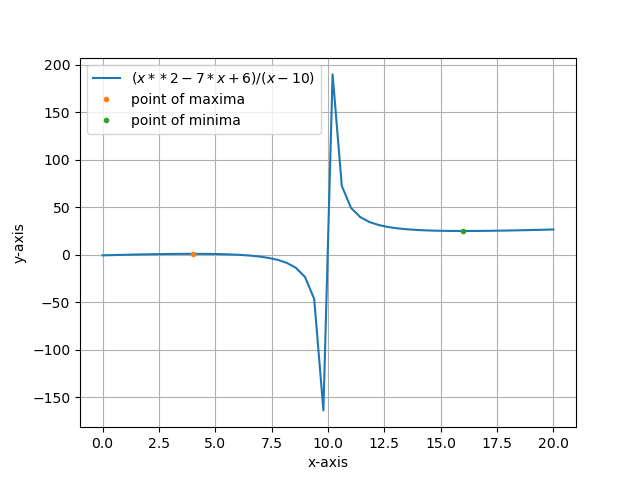
\includegraphics[width=1\columnwidth]{optA.png}
\caption{Plot of f(x) to find Maxima and Minima}
\label{Optimization of Machince A and B}
\end{figure}

\section{Conclusion}
\begin{flushleft}
1. At first, the given function has been differentiated and it is solved by setting f'(x) equal to zero. By using x values, f(x) values are calculated.\\
\vspace{0.25cm}
2. Later, the given function f(x) is solved by gradient ascent algorithm to find maxima and the point at which f(x) is maximum.\\
\vspace{0.25cm}
3. Then, the given function f(x) is solved by gradient descent algorithm to find minima and the point at which f(x) is is minimum.\\
\vspace{0.25cm}
4. Maxima and Minima and related points are, \\
\vspace{0.25cm}
\center
Maxima point, Max=(4 , 1) and\\ 
\vspace{0.2cm}
Minima point, Min=(16 , 25)
\end{flushleft}
\endcenter
\end{flushleft}
\end{document}
